\documentclass[utf8,xcolor=table, page number]{earlywinter}

\usepackage[T1]{fontenc}
\usepackage[frenchb]{babel}
\usepackage{graphicx}

\begin{document}
\title{Edge Cloud Computing}
\author{Aurèle BARRIÈRE & Solène MIRLIAZ}

\begin{frame}[plain]
  \titlepage%
\end{frame}

% ----------------
% - Introduction -
% ----------------
\section{Introduction}
\begin{frame}
	\frametitle{Introduction}

\end{frame}

  \begin{frame}
    \frametitle{Table of contents}
    \tableofcontents[]
  \end{frame}
  
  
\section{Edge computing challenges}
\subsection{A new model will be needed}
\begin{frame}
  \frametitle{\subsecname}
  \begin{block}{Internet of things}
    Growth of the number of connected objects and sensors that generate data.
    The end nodes are evolving from consumers to producers.
    
    Estimated produced data by 2019: 500 zettabytes (estimate by Cisco Global Cloud Index).
  \end{alertblock}
	\begin{alertblock}{Limits of the clouds}
          \begin{itemize}
          \item The network can't handle that much.\\
              Estimated IP traffic by 2019: 10.4 zettabytes.
	    \item For many uses (multimedia for instance), the Cloud introduces too much latency.
          \end{itemize}
	\end{alertblock}

\end{frame}

\subsection{Bringing the cloud to the Edge: an hybrid system} %I'm not sure this is a good phrasing. maybe some of the papers we read would disagree
\begin{frame}
  \frametitle{Edge computing}
  \framesubtitle{Principle}

  \begin{block}{Computing in the Edge}
    Increase in the nodes' computing power as well (smartphones, embedded devices).
  \end{block}
   We want to put computing at the proximity of data sources: at the Edge.
  

\end{frame}

\begin{frame}
  \frametitle{Edge-Cloud computing}
  \framesubtitle{An hybrid system}

  \begin{figure}
    \center
    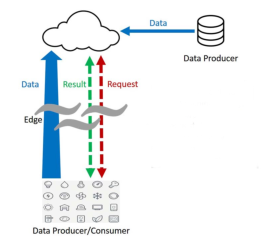
\includegraphics[scale=0.5]{edge.png}  %I'm not a big fan of this graphic. might have to change it.
  \end{figure}

  Keep using the Cloud (core), but add computation at the Edge.
  The Cloud keeps providing global services, but edge servers can compute with lower latency.
  
\end{frame}

\subsection{Challenges}

% the challenges and research interests are almost the same to me

\begin{frame}
  \frametitle{Challenges}
  \framesubtitle{Energy}
  
  Mobile device with low battery
  
\end{frame}
\begin{frame}
  \frametitle{Challenges}
  \framesubtitle{Computing power}
  
  Increasing
  
\end{frame}
\begin{frame}
  \frametitle{Challenges}
  \framesubtitle{Mobility}
  
  Mobile things. Failure-tolerence must be high.
  
  Where to put the service in the edge?
  
\end{frame}
\begin{frame}
  \frametitle{Challenges}
  \framesubtitle{Heterogenity}
  
  Of the network and things' abilities.
  
	\begin{example}
		Cellphone, Oven, radio, heater, computer, etc.
	\end{example}
  
  Of the programming languages used by each.  
  
  Of the applications
	\begin{example}
		High CPU need, high memory need, quick communication, etc.
	\end{example}
  
\end{frame}

\section{Current research studies}
\subsection{Architecture}
\begin{frame}
  \frametitle{Current Research}
  \framesubtitle{Architecture}
\end{frame}
\subsection{Workload Distribution}
\begin{frame}
  \frametitle{Current Research}
  \framesubtitle{Workload Distribution}
\end{frame}
\subsection{Problem Identification and Heuristics}
\begin{frame}
  \frametitle{Current Research}
  \framesubtitle{Problem Identification and Heuristics}
  \begin{exampleblock}{On-demand gaming coverage} % [4]
    We need a low-latency service that can satisfy the most people.\\
    We need heuristics for edge servers deployment.
  \end{exampleblock}
\end{frame}
\subsection{Programmability}
\begin{frame}
  \frametitle{Current Research}
  \framesubtitle{Programmability}
\end{frame}
\subsection{Naming}
\begin{frame}
  \frametitle{Current Research}
  \framesubtitle{Naming}
\end{frame}

\section{Case example: a traffic light}
\begin{frame}
  \frametitle{Case Example}
  \framesubtitle{Smart Traffic Light}
\end{frame}
\section{Conclusion}
\begin{frame}
  \frametitle{Conclusion}
  Hybrid system needed.
  No cure-all solution.
  
  What about the economical aspect ?
  
\end{frame}
\end{document}
